\documentclass[letterpaper,12pt]{article}
\usepackage{tabularx} % extra features for tabular environment
\usepackage{amsmath}  % improve math presentation
\usepackage{graphicx} % takes care of graphic including machinery
\usepackage{listings}
\usepackage{minted}
\usepackage[margin=1in,letterpaper]{geometry} % decreases margins
\usepackage{cite} % takes care of citations
\usepackage[final]{hyperref} % adds hyper links inside the generated pdf file
\hypersetup{
	colorlinks=true,       % false: boxed links; true: colored links 
	linkcolor=blue,        % color of internal links
	citecolor=blue,        % color of links to bibliography
	filecolor=magenta,     % color of file links
	urlcolor=blue         
}

\lstset{ 
  frame=none,   
  xleftmargin=2pt,
  stepnumber=1, 
  numbers=left,
  numbersep=5pt,
  numberstyle=\ttfamily\tiny\color[gray]{0.3},
  belowcaptionskip=\bigskipamount,
  captionpos=b,
  escapeinside={*'}{'*},
  language=haskell,  
  tabsize=2,
  emphstyle={\bf},
  commentstyle=\it,
  stringstyle=\mdseries\rmfamily, 
  showspaces=false,
  keywordstyle=\bfseries\rmfamily,
  columns=flexible,
  basicstyle=\small\ttfamily, %sffamily,
  showstringspaces=false,
  morecomment=[l]\%,
}

\begin{document}

\title{Machine Problem 1: Decision Tree with Categorical and Real Valued Attributes}
\author{John L. Singleton}
\date{\today}
\maketitle

%% \begin{abstract}
%%   We present the implementation of a decision tree classifier with categorical and real valued attributes. Using a data set containing information about the Miles Per Gallon ratings for 398 cars, we constructed a classifier capable of correctly deciding if a given instance was able to achieve a fuel efficiency greater than 20 miles per gallon.
  
%% \end{abstract}

\section{Problem Selection}

For our experiment, we chose to build a decision tree classifier with a data set containing information about the Miles Per Gallon ratings for 398 different cars. The goal of this experiment was to train the classifier to be able to decide if a given instance (formulated in terms of the attributes defined in section 2) will be able to achieve greater than 20 miles per gallon efficiency.

\section{Data Set Selection and Characteristics} 

The data set we chose to work with for this project was the Auto MPG data set \cite{Lichman:2013} which can be obtained from the following URL: \href{http://archive.ics.uci.edu/ml/datasets/Auto+MPG}{http://archive.ics.uci.edu/ml/datasets/Auto+MPG}.

The MPG dataset is a multivariate data set containing both categorical and real valued attributes. The attributes of this data set that are relevant to our experiment are detailed in Table \ref{table:dataset}.

\begin{table}[H]
  \centering
\begin{tabular}{ | l | c | c | c | c | c |}
  \hline
  Attribute & Type & Average & Min & Max & $\sigma$ \\
  \hline
  \hline
  Cylinders & Real  &  5.47 & 3 & 8 & 1.70 \\
  \hline
Displacement & Real  &  194.41 & 68 & 455 & 104.64 \\
  \hline
Horsepower & Real  &  104.46 & 46 & 230 & 38.49 \\
  \hline
Weight & Real  &  2977.58 & 1613 & 5140 & 849.40 \\
  \hline
Acceleration & Real  &  15.54 & 8 & 24.8 & 2.75 \\
  \hline
Year & Real  &  75.97 & 70 & 82 & 3.68 \\
  \hline
Origin & Real  &  1.57 & 1 & 3 & 0.80 \\
  \hline
  Model & Categorical  &  - & -  & -  & - \\
  \hline
  Total Samples: & 398 & & & & \\
  \hline
  Usable Samples: & 392 & & & & \\
  \hline
\end{tabular}
\caption{Attributes of the MPG data set.}
\label{table:dataset}
\end{table}

For our experiment all examples were considered except for 6, which were unusable due to missing data. These samples were filtered out of our data set and not used. 

\section{K-Fold Validation of Data Set}

For the K-Fold validation of our data set, we chose to allow the data set to be split automatically at runtime. There are a few important aspects to this splitting. First, to minimize bias of performing a k-fold validation on the same (deterministic) folds, we randomize our list. For all experiments performed in this paper, \textbf{we chose a K value of 3 resulting in validation set sizes of 130.} As noted in the previous section, the entire data set size contained 392 examples. Every permutation of training set with cross validation set was performed, resulting in 3 training and validation trials. We provide a sample of our k-fold implementation in Listing \ref{code:kfold}.

\begin{listing}[H]
\begin{minted}
[frame=lines,
framesep=2mm,
fontsize=\footnotesize
]
{haskell}
validate :: (LoadableModel a) =>
  [a]                            -- examples
  -> ([a] -> StopCondition)      -- purity function
  -> ([a] -> [AttributeGroup a]) -- the attribute builder
  -> Int                         -- number of sets
  -> (a -> Bool)                 -- category function 
  -> IO ClassifierAccuracy
validate examples purityFunction decisionTreeAttributes k categoryFunction = do
  examples' <- shuffle examples
  let parts = trace ("Validating with k=" ++ (show k)) (split examples' k)
  let perms = permutations parts
  c <- makeCounter
  scores <- mapM (\(validationModel:trainingSets)-> do
           let trainingModel = trace ("Validating Model...") $ concat trainingSets
           let attributes = decisionTreeAttributes trainingModel
           tree <- buildTree NoAttribute attributes trainingModel purityFunction 0 c
           return (score validationModel tree categoryFunction)) perms
            
  -- average the scores
  return $ rollup scores
\end{minted}

\caption{K-Fold Cross Validation in \texttt{Classifier.hs}. Note that prior to splitting the list, the list is randomized.}
\label{code:kfold}
\end{listing}

\section{Decision Tree Implementation}
For our experiments we chose to implement the decision tree classifier in the Haskell programming language. The source code of our implementation (along with this report) is available at the following URL: \href{https://github.com/jsinglet/decision-tree-classifier}{https://github.com/jsinglet/decision-tree-classifier}. The details of compiling and running this project are given in Section \ref{sec:reproduction}.

\subsection{Selecting Attributes}

At each tree split point, an attribute must be chosen to classify on. For our implementation we enforced the restriction that for any subtree, a given attribute may only be selected once. This scenario allows for a given attribute to be selected in orthogonal trees, but prevents it from happening in the same subgraph in order to minimize overfitting.
 
At each split point, the best possible attribute was selected by calculating the GINI index \cite{aggarwal_data_2015} of each attribute for a given subset of examples and then selecting that attribute. We take the GINI index to be given by Equation \ref{eqn:gini}.

\begin{equation}
  G(v_i) = 1 - \sum_{j=1}^k p_j^2
  \label{eqn:gini}
\end{equation}

  
We provide the relevant code for this operation in Listing \ref{code:gini}.
   
\begin{listing}[H]
\begin{minted}
[frame=lines,
framesep=2mm,
fontsize=\footnotesize
]
{haskell}



classify ::
  AttributeGroup a
  -> [a]
  -> [(Attribute a, [a])]
classify (AttributeGroup _ _ attributes)  examples =
  map (\attribute@(AttributeClassification _ _ f) ->
         (attribute, filter f examples)
      ) attributes

-- we select the attribute that would produce the lowest gini index. 
selectAttribute ::
  [AttributeGroup a]
  -> [a]
  -> Int
  -> ([AttributeGroup a], AttributeGroup a)
selectAttribute attrs examples d = do
  let indexed = map (\x ->
                       ((calculateGini (classify x examples) examples ), x)
                    ) attrs
  let (lowestGiniIndex, a) = foldr (\acc x ->
                                      if fst x < fst acc then
                                        x
                                      else acc)
                             (head indexed) indexed
  let remainingAttributes = filter (\x@(AttributeGroup _ name _)  ->
                                      let (AttributeGroup _ name2 _) = a in name /= name2)
                            attrs
  (remainingAttributes, a)

calculateGiniIndex classified examples pf =
  weightedAverage $
  map (\(_, classifiedExamples)
       ->  (fromIntegral $
       length classifiedExamples) *
       (1 - ((c1 classifiedExamples)^2  +  (c2 classifiedExamples)^2)) -- Sigma
      ) classified
  where
    c1 ex = case (pf ex) of
      Yes -> 1.0
      No  -> 0.0
      CantSay d -> d
    c2 ex = case (pf ex) of
      Yes -> 0.0
      No  -> 1.0
      CantSay d -> 1.0-d
    weightedAverage x = Stats.mean x
                            
\end{minted} 

\caption{Implementation of GINI minimization function in \texttt{DecisionTree.hs}}
\label{code:gini} 
\end{listing}

 
\subsection{Splitting Attributes}

Since none of the attributes in our data set are binary, one of the first challenges of this project was to devise an optimal splitting strategy for both the real and categorical attributes. For real attributes, we allowed the split points to be determined at runtime based on an examination of the training data set.

For each real-valued attribute, the split point was derived by computing the minimization function given in Equation \ref{eqn:min}.

\begin{equation}
  \min_{j,s} \left[\sum_{x_i \in R_1(j,s)} (x_i - \hat\beta_1)^2 + \sum_{x_i \in R_2(j,s)} (x_i - \hat\beta_2)^2\right]
  \label{eqn:min}
\end{equation} 

Where $R_1$ consists of the set of values less than or equal to some split point $s$ and $R_2$ is the set of values that are greater than some split point $s$. The values $\hat\beta_1$ and $\hat\beta_2$ are given by:

\[
\hat\beta_1 = avg(y_i ~|~ x_i \in R_1(j,s)))
\]
\[
\hat\beta_2 = avg(y_i ~|~ x_i \in R_2(j,s)))
\]

We provide the details of our implementation of this minimization function in Listing \ref{code:two}.

For our data set we only needed to split one categorical attribute: the car model. Typically the car model data was formatted in the following way:

\begin{center}
  [car-make] [model identifier]
\end{center}

For example, ``toyota camry." Because the car manufacturer is likely to contain more information than the model name (which is generally of little technical significance), we chose to split the car model attribute based on manufacturer. This resulted in 37 unique categories for this attribute. 

\begin{listing}[H]
\begin{minted}
[frame=lines,
framesep=2mm,
fontsize=\footnotesize
]
{haskell}
data MinimizationResult a =
  MinimizationResult (a, a)   -- MinimizationResult (whereToSplit, minimizationResult)
  | NoResult                  -- For the initial minimization
  deriving (Show)

minimize ::  (Fractional a, Ord a) =>
             [a]
             -> MinimizationResult a
             -> [a] 
             -> MinimizationResult a
minimize d res (s:ss) =
  case (res) of
  NoResult -> minimize d (MinimizationResult (s, sigmaTerm)) ss
  MinimizationResult (_, splitVal) ->
    if sigmaTerm < splitVal then
      minimize d (MinimizationResult (s, sigmaTerm)) ss
    else minimize d res ss

  where
      sigmaTerm = sum t1 + sum t2
      r1 = [ x | x <- d, x <= s]
      r2 = [ x | x <- d, x >  s]
      b1 = mean r1
      b2 = mean r2
      -- the left and right term
      t1 = [ (x - b1)*(x - b1) | x <- r1]
      t2 = [ (x - b2)*(x - b2) | x <- r2]

minimize d res [] = res
\end{minted}
\label{code:two}
\caption{Implementation of minimization function in \texttt{Minimize.hs}}
\end{listing}


\subsection{Stopping Criteria}

For stopping criteria we elected to stop on either of the following conditions:

\begin{enumerate}
  \item Once all of the instances at a given node belonged to the same classification (yes or no).
  \item When the tree depth reached 8 levels, that is, once it has exhausted attributes to classify on in a given subtree. 
\end{enumerate}

In our design, if a search ``bottoms out" by reaching the maximum of 8 levels, we assign a category of \texttt{CantSay} to the leaf, and calculate the purity of that node as the percentage of samples in the classification at point. If the sample is greater than 50\%, we declare a guess of ``yes." Otherwise we classify that node as a ``no." Note that in our model the tree reaches the 8 levels simply by exhausting the attributes to classify on. Since we constrain each subtree to only select an attribute once, the maximum height of our entire tree is only 8.

\section{Reproducing this Experiment}
\label{sec:reproduction}
To compile, you will need a curent installation of Haskell Platform,
which can be obtained from here: \href{https://www.haskell.org/platform/}{https://www.haskell.org/platform/}.

Then, you can build this project by entering the following commands:
\begin{listing}[H]
\begin{minted}
[frame=lines,
framesep=2mm,
fontsize=\footnotesize
]
{bash}
$ cabal sandbox init
$ cabal install
\end{minted}
\end{listing}

The resulting executable will be palced at \texttt{.cabal-sandbox/bin/decision-tree-classifier}.

After you build \texttt{decision-tree-classifier}, you can run it as follows,
from the root of the source directory. To perform a k-fold validation,
run the following command. 

\begin{listing}[H]
\begin{minted}
[frame=lines,
framesep=2mm,
fontsize=\footnotesize
]
{bash}
$ .cabal-sandbox/bin/decision-tree-classifier -validate
\end{minted}
\end{listing}

To output the internal representation of the graph in DOT (GraphViz)
format, use the following command:
\begin{listing}[H]
\begin{minted}
[frame=lines,
framesep=2mm,
fontsize=\footnotesize
]
{bash}
$ .cabal-sandbox/bin/decision-tree-classifier -show
\end{minted}
\end{listing}

In addition to the options shown above, this tool also supports a \texttt{-check} option that evaluates the training set against a validation set for purposes of doing quick overfitting checking. 


\section{Results}
 

In this section we present the results of our decision tree classifier. In our $k=3$ fold validation we observed that our classifier achieved the performance as documented in Table \ref{table:with-model}. For illustration purposes, we also show the internal representation of our decision tree classifier in Figure \ref{fig:tree}. Note that the tree pictured in \ref{fig:tree} does not include the car make attribute; due to the highly dimensional nature of this attribute the resulting graph that is generated cannot be easily displayed visually. 

\begin{figure}[H]
  \makebox[\linewidth]{
    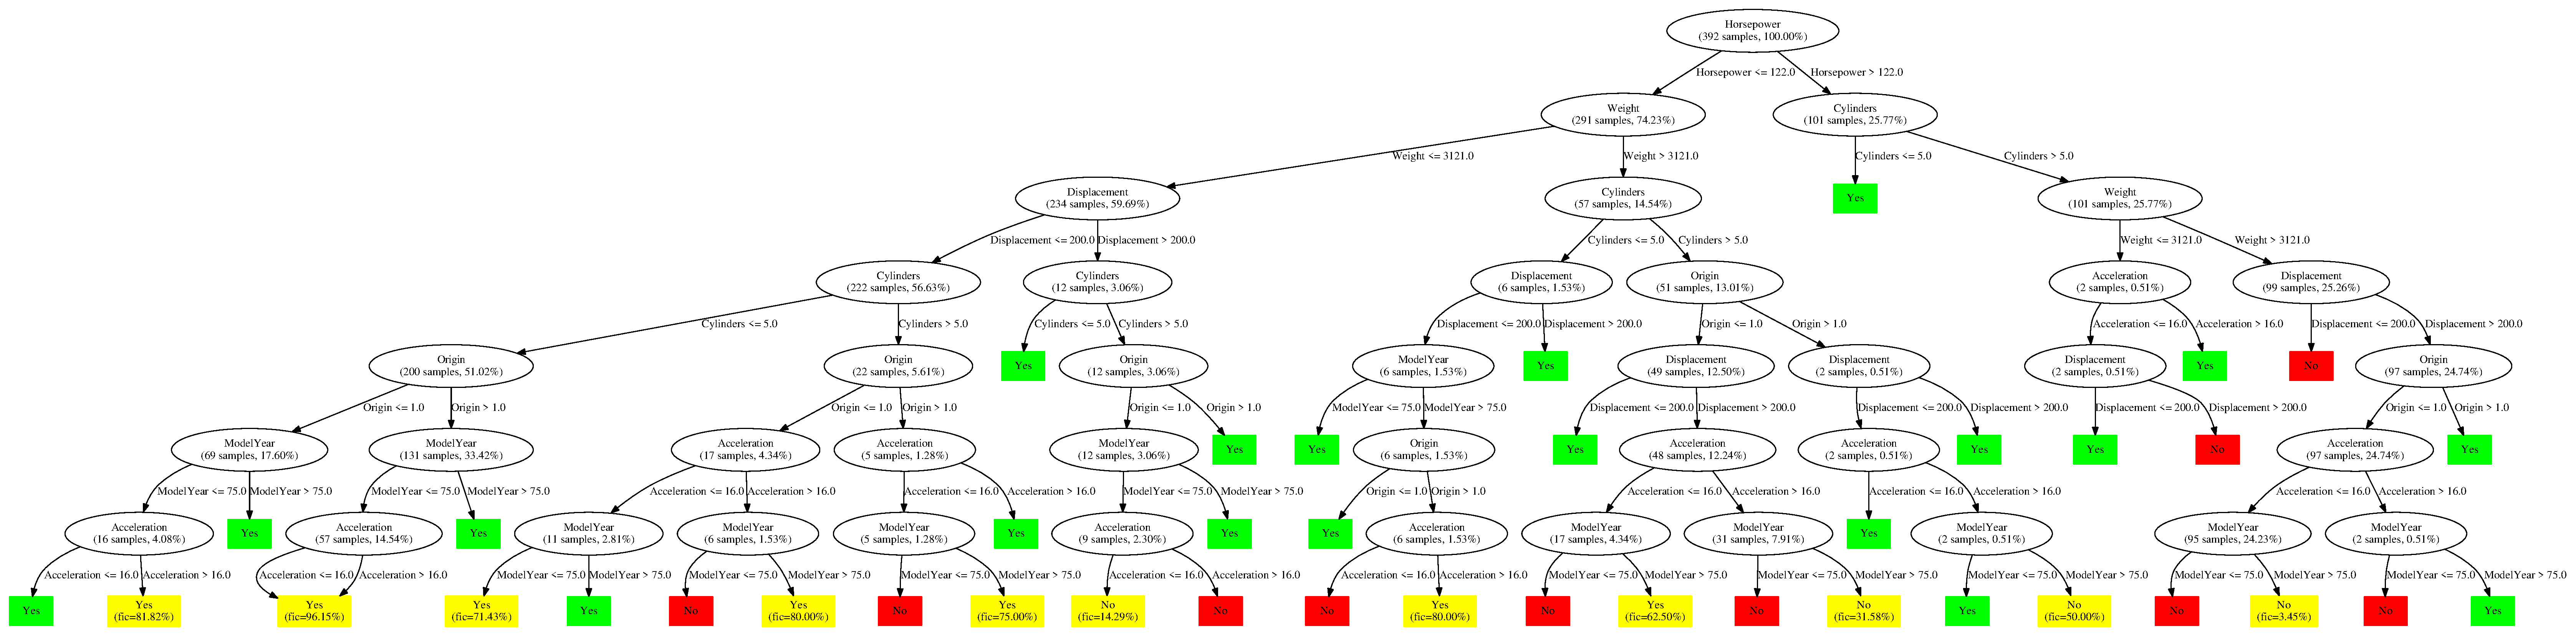
\includegraphics[scale=.15]{../run2.eps}
    }
  \caption{A graphical representation of our decision tree classifier generated by a classification run that excluded the model information of our data set. In our figure, the yellow nodes represent non-pure decisions and the red and green nodes represent nodes where the purity of the samples is 100\%.}
  \label{fig:tree}
\end{figure}



\begin{table}[H]
  \centering
\begin{tabular}{ | l | c | c | c |}
  \hline
  Attribute &  Average & Median & $\sigma$ \\
  \hline
  Precision & 0.869 & 0.855 & 0.029 \\
  \hline
  Recall  &   0.891 & 0.894 & 0.032 \\ 
  \hline
  FMeasure &  0.879 & 0.88 & 0.078 \\
  \hline
  Accuracy & 0.856 & 0.861 & 0.008 \\
  \hline
\end{tabular}
\caption{Classifier accuracy report with a model that includes the car make attribute.}
\label{table:with-model}
\end{table}




\begin{table}[H]
  \centering
\begin{tabular}{ | l | c | c | c |}
  \hline
  Step & Accuracy & FMeasure & Error \\
  \hline
  1 & .861 & .88 & .318\\
  \hline
  2    & .846 & .871 & .153 \\
  \hline
  3  & .861 & .887 & .138 \\
  \hline
\end{tabular}
\caption{Classifier accuracy report by each step of k-cross fold validation.}
\label{table:with-model}
\end{table}


A few interesting aspects are evident in Table \ref{table:with-model}. First, our classifier demonstrates a FMeasure of $.87$, with a standard deviation of approximately .078. Though the results of our cross validation displayed stable performance with unseen data, we conducted one final measure to check for overfitting. In this test we simply split our data set into two parts. We trained our decision tree on one half of the data and then used the resulting decision tree to score the data that had been used to train it. To see if perhaps the tree was too closely learning the training data we then used the unseen data on the trained decision tree and compared the results. The data from this experiment is displayed in Table \ref{table:overfitting}. 

\begin{table}[H]
  \centering

  \begin{tabular}{l|l|l|}
\cline{2-3}
                                & \textbf{Trained Data} & \textbf{Unseen Data} \\ \hline
\multicolumn{1}{|l|}{Precision} & 0.982                 & 0.941                \\ \hline
\multicolumn{1}{|l|}{Recall}    & 0.982                 & 0.937                \\ \hline
\multicolumn{1}{|l|}{FMeasure}  & 0.982                 & 0.923                \\ \hline
\multicolumn{1}{|l|}{Accuracy}  & 0.979                 & 0.923                \\ \hline
\end{tabular}
\caption{Comparison of trained decision tree performance on trained vs unseen data.}
\label{table:overfitting}
\end{table}

As can be seen in  Table \ref{table:overfitting}, the trained data predictably performs better than the unseen data. However, this is by a very small margin (less than 0.10 in all cases). As can been seen in the cross validation results the decision tree classifier indeed does generalize to unseen data since each step of the k-fold validation achieves greater than .85 in each category of performance. 

\bibliography{report}
\bibliographystyle{plain}

\end{document}
